\documentclass[12pt,a4paper]{article}
\usepackage{amsmath}
\usepackage{amsfonts}
\usepackage{amssymb}
\usepackage{graphicx}
\usepackage{secdot}
\usepackage[left=2cm,right=2cm,top=2cm,bottom=2cm]{geometry}

\author{Shibayan Biswas, AE21B109\\ Department of Aerospace Engineering\\ IIT Madras}

\title{Assignment - 2}

\date{September 07, 2022}

\begin{document}

\maketitle
\hline
\section{Gaussian Elimination for Matrices:}
In mathematics, Gaussian elimination, also known as row reduction, is an algorithm for solving systems of linear equations. It consists of a sequence of operations performed on the corresponding matrix of coefficients. This method can also be used to compute the rank of a matrix, the determinant of a square matrix, and the inverse of an invertible matrix. The method is named after Carl Friedrich Gauss.  
\subsection{Methods for Finding Solution Matrix:}
In this particular section I have provided the different methods by which we can find the solution of a Matrix in Octave. In mathematics, Gaussian elimination, also known as row reduction, is an algorithm for solving systems of linear equations. It consists of a sequence of operations performed on the corresponding matrix of coefficients. This method can also be used to compute the rank of a matrix, the determinant of a square matrix, and the inverse of an invertible matrix. The method is named after Carl Friedrich Gauss (1777–1855) although some special cases of the method—albeit presented without proof—were known to Chinese mathematicians as early as circa 179 AD.
\subsubsection{Method- 1 (Gaussian Elimination Method):}
This is the most elementary method to find the solutions of a system of linear equations using the Gaussian elimination method. This method takes the maximum wall clock time out of the three methods that we have represented in our report. It consists of a sequence of operations performed on the corresponding matrix of coefficients. This method can also be used to compute the rank of a matrix, the determinant of a square matrix, and the inverse of an invertible matrix.
\subsubsection{Method- 2 (Inverse Matrix Method):}
This method of solving the linear equations is more efficient than the previous method and it takes less wall clock time compared to the previous method. In this method we use the "inverse" inbuilt function for finding the inverse of a matrix.\\
\subsubsection{Method- 3 (Using pinv ($\backslash$) operator):}
This is the most efficient method for solving the system of linear equations among the all three methods using the pinv ($\backslash$)  operator. This method consumes the least wall clock time for computing compared to the other two methods that we have discussed previously.
\subsection{Plot of L$\infty$ vs n:}
In this particular section the plot of the L$\infty$ norm of error between the Method 1 and Method 2 and Method 1 and Method 3 against matrix size 'n' up to 1000 is shown below in the figure:
\begin{figure}[!ht]
	\begin{center}
		\framebox{
			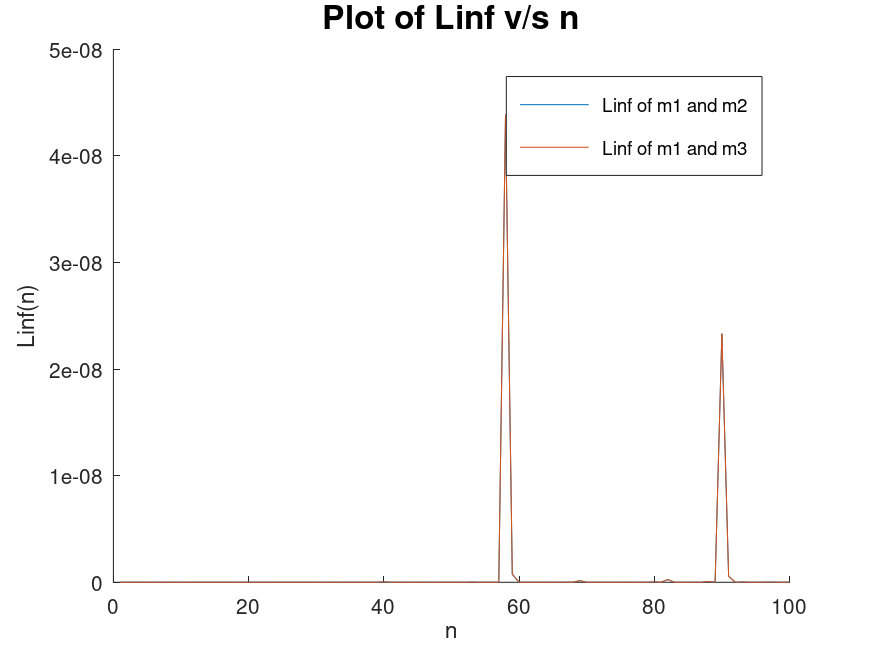
\includegraphics[scale=0.5]{Linf.png}
		}
	\end{center}
	\caption{L$\infty$ plot}
	\label{L∞ plot}
\end{figure}
\subsection{Wall Clock Time for all Methods:}
In this section I have shown the plot for the wall clock time for each method discussed in the previous sections. Wall time, also called real-world time or wall-clock time, refers to elapsed time as determined by a chronometer such as a wristwatch or wall clock. (The reference to a wall clock is how the term originally got its name.) Wall time differs from time as measured by counting microprocessor clock pulses or cycles. .The required plot is shown below in the figure:
\clearpage
\begin{figure}[!ht]
	\begin{center}
		\framebox{
			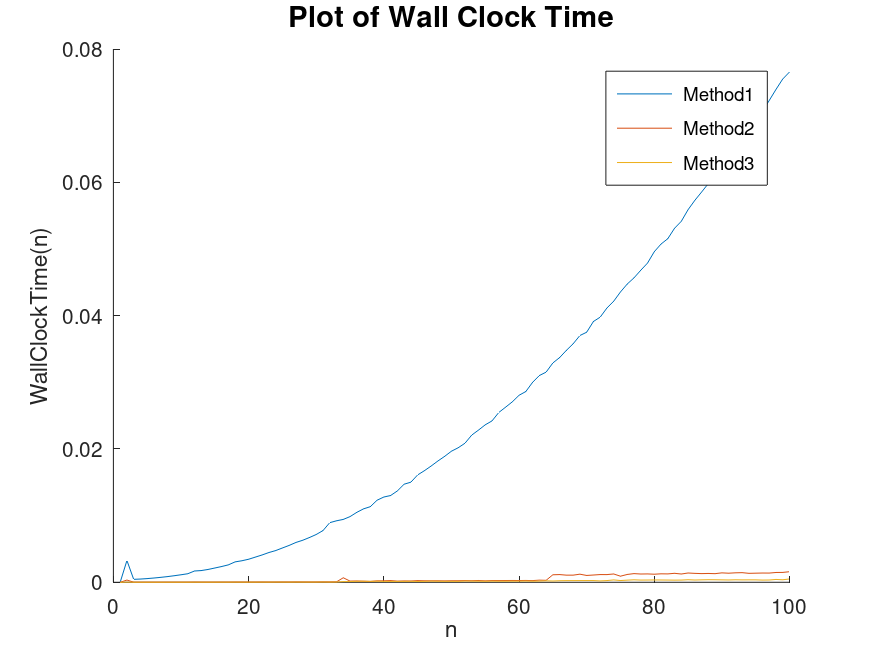
\includegraphics[scale=0.5]{WLC.png}
		}
	\end{center}
	\caption{Wall-clock time plot}
	\label{wall-clock time plot}
\end{figure}

\section{Regression Analysis:}
Linear regression analysis is used to predict the value of a variable based on the value of another variable. The variable you want to predict is called the dependent variable. The variable you are using to predict the other variable's value is called the independent variable.
\subsection{A brief overview on Linear Regression:}
Linear regression is a basic and commonly used type of predictive analysis.  The overall idea of regression is to examine two things: \\
(1) Does a set of predictor variables do a good job in predicting an outcome (dependent) variable? \\ 
(2) Which variables in particular are significant predictors of the outcome variable, and in what way do they–indicated by the magnitude and sign of the beta estimates–impact the outcome variable? \\
These regression estimates are used to explain the relationship between one dependent variable and one or more independent variables. 
\subsection{Performing Regression Analysis on the Data Sets given:}
Here we have performed Regression Analysis on the data sets given in the assignment template and we get the following plots for the best fit line for each data set provided to us. We have used Regression to predict the value of a variable based on the value of another variable. The variable you want to predict is called the dependent variable. The variable you are using to predict the other variable's value is called the independent variable.
\begin{figure}[!ht]
	\begin{center}
		\framebox{
			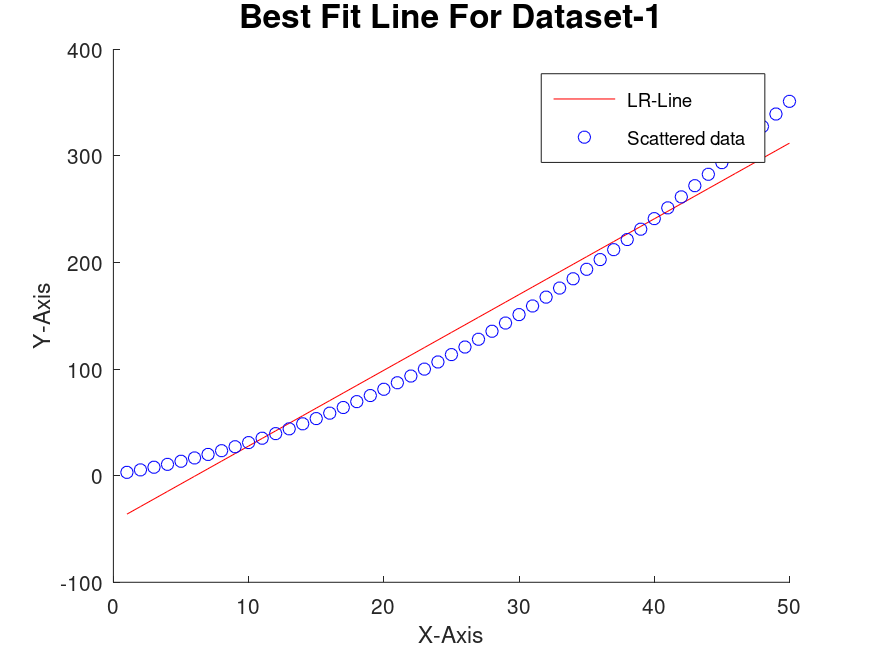
\includegraphics[scale=0.4]{lrd1.png}
		}
	\end{center}
	\caption{Regression plot for data set 1}
	\label{Regression plot for data set 1}
\end{figure}
\begin{figure}[!ht]
	\begin{center}
		\framebox{
			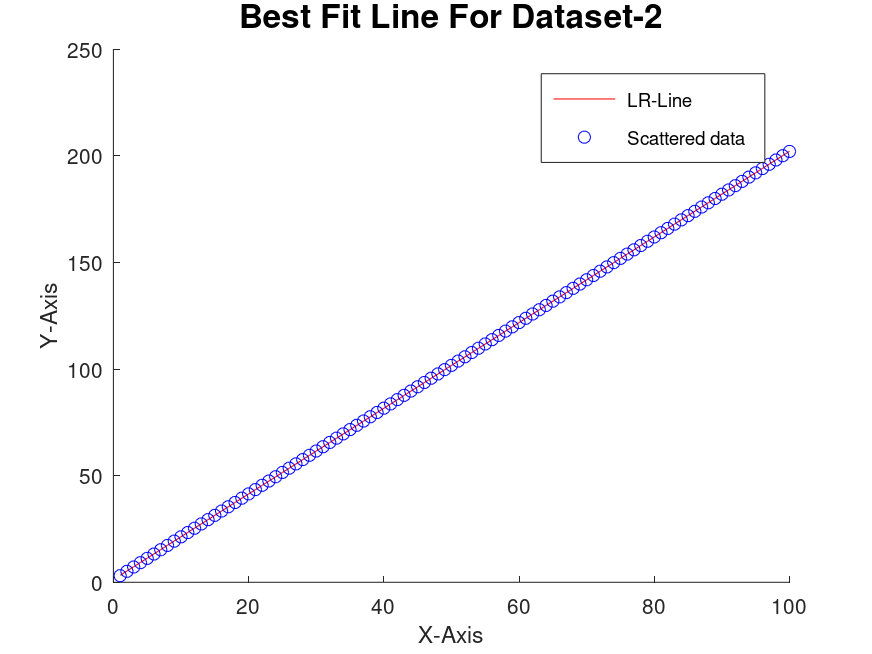
\includegraphics[scale=0.4]{lrd2.png}
		}
	\end{center}
	\caption{Regression plot for data set 2}
	\label{Regression plot for data set 2}
\end{figure}
\begin{figure}[!ht]
	\begin{center}
		\framebox{
			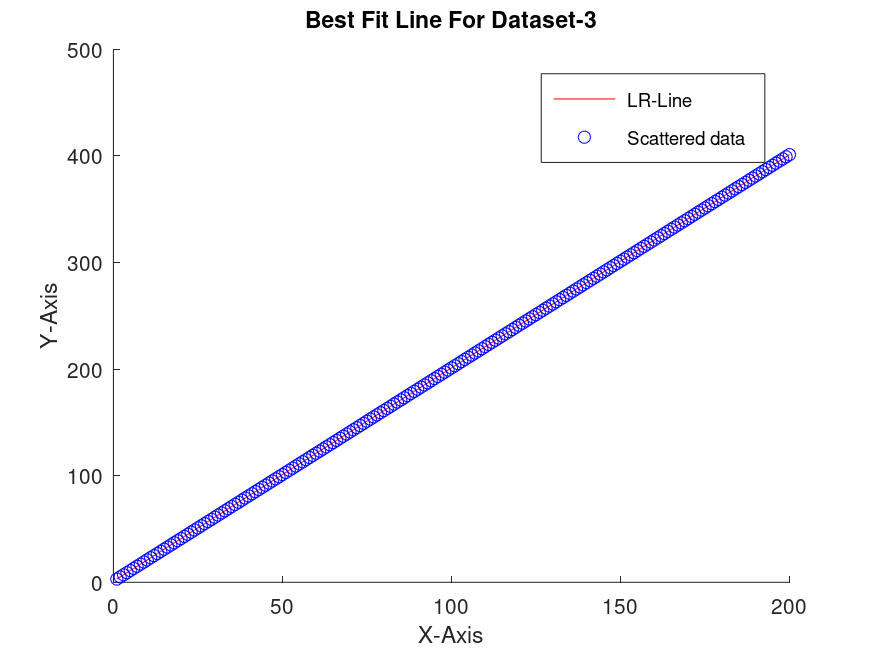
\includegraphics[scale=0.4]{lrd3.png}
		}
	\end{center}
	\caption{Regression plot for data set 3}
	\label{Regression plot for data set 3}
\end{figure}
\subsection{Tables for the data sets:}
In this section we have represented the output tables for the data sets where the rows are 50, 100, 200 and the columns indicate the values of m and c, and based on the values, we infer that the nature of the data provided for the $1^{st}$ data set; when the rows increase there is a drastic change in the values of 'm' and 'c' compared to the other two data sets which represent a more linear variation. We confirm the statement from the result of the Regression Analysis performed on the given data sets represented in the previous subsection. 
\begin{table}[h]
	\begin{center}
\begin{tabular}{|c|r|l|}
\hline
Rows & m & c \\
\hline
50 & 7.1000 & -43.2000 \\
100 & 12.1000 & -170.7000 \\
200 & 22.1000 & -675.7000 \\
\hline
\end{tabular}
	\caption{Output Table for $1^{st}$ data set}
	\label{tab:progs}
	\end{center}
\end{table}
\begin{table}[h]
	\begin{center}
\begin{tabular}{|c|r|l|}
\hline
Rows & m & c \\
\hline
50 & 2.0111 & 1.1956 \\
100 & 2.0079 & 1.2719 \\
200 & 2.0056 & 1.3810 \\
\hline
\end{tabular}
	\caption{Output Table for $2^{nd}$ data set}
	\label{tab:progs}
	\end{center}
\end{table}
\clearpage
\begin{table}[h]
	\begin{center}
\begin{tabular}{|c|r|l|}
\hline
Rows & m & c \\
\hline
50 & 2.0000 & 1.0049 \\
100 & 2.0000 & 1.0047 \\
200 & 2.0000 & 1.0050 \\
\hline
\end{tabular}
	\caption{Output Table for $3^{rd}$ data set}
	\label{tab:progs}
	\end{center}
\end{table}
\subsection{Best Fit Curve for Data Set- 1:}
The model that would work for the $1^{st}$ data set instead of a linear curve is a best fit curve (non-linear) because the the variation of the Regression analysis performed on data set 1 is not linear. Hence the hypothesis for the given model is proved.
\begin{figure}[!ht]
	\begin{center}
		\framebox{
			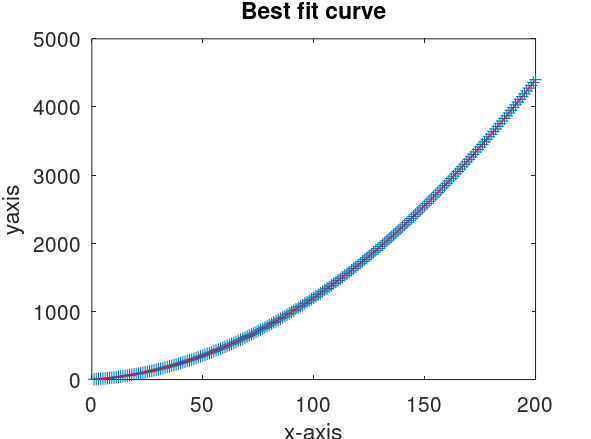
\includegraphics[scale=0.6]{hw2_2_5_best_fit.png}
		}
	\end{center}
	\caption{Best fit curve for data set 1}
	\label{Best fit curve for data set 1}
\end{figure}
\end{document}